\chapter{Results and Discussion}



\section{Segmentation results}
Figure~\ref{fig:Segmentation sample}displays a sample of the segment maps generated using SLIC. Our aim was to produce homogeneous segments by testing various combinations of compactness and the number of segments parameters.
 \begin{figure}[h]
    \centering
    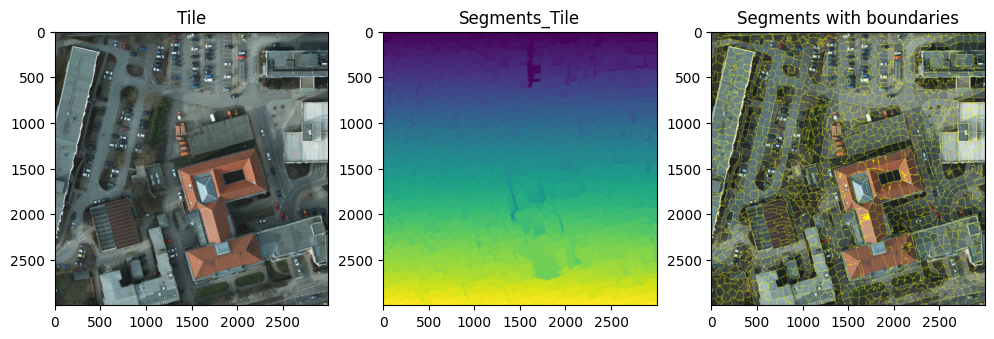
\includegraphics[width=1\linewidth]{images/Segmentation sample.png}
    \caption{Exemplary segmentation obtained using the SLIC algorithm with the following parameters {n\_segments=1800,compactness=0.1}}
    \label{fig:Segmentation sample}
\end{figure}

The percentage purity, which measures the proportion of segments containing only a single class label, was evaluated for the training, validation, and testing samples. Initial experimentation resulted in an average of 1250 segments per image, with segments having at least 90\% class purity amounting to 47\% of the testing set and 41\% of the training set.


Ensuring that segments accurately represent the underlying classes in the dataset is crucial for accurate classification. However, it was observed that small objects, particularly the car class, were not adequately represented when computing the majority label for each segment.



\section{Random Forest}
The feature engineering process generated a combination of forty-eight textural, geometric, and spectral features. These features were used to train the random forest model. At testing,the model performed relatively well in distinguishing impervious surfaces and clutter, and it showed acceptable performance with buildings and low vegetation. However, the model struggled to identify trees and cars as illustrated in the lower F1 scores in Figure \ref{tab:RF_F1}. This difficulty stems from class imbalance as illustrated on the confusion matrix, which while it was addressed by computing weighted F1 scores for each class, still did not do well. 
\begin{figure}[h]
    \centering
    \begin{minipage}[b]{0.45\linewidth}
        \centering
        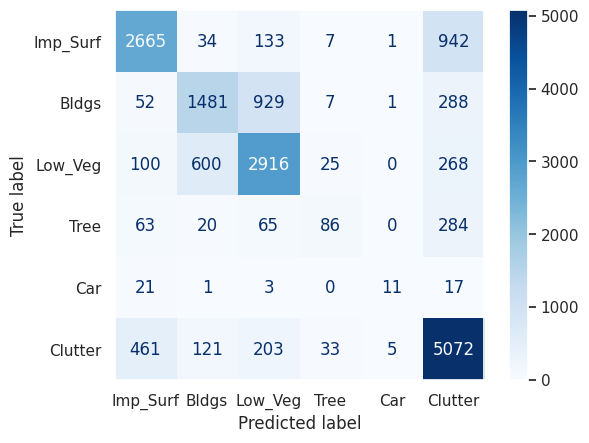
\includegraphics[height=5cm]{images/RF Confusion matrix.png} % Adjust the height as needed
        \caption{Random Forest Confusion Matrix}
        \label{fig:RF_CM}
    \end{minipage}
    \begin{minipage}[b]{0.45\linewidth}
        \centering
        \begin{tabular}{c|c|c|c|c}
        \hline
             Class & Precision & Recall & F1-Score & Support \\
             \hline
             Imp\_surf & 0.79 & 0.70 & 0.75 & 3782 \\
             Bldgs & 0.66 & 0.54 & 0.59 & 2758 \\
             Low\_Veg & 0.69 & 0.75 & 0.71 & 3909 \\
             Tree & 0.54 & 0.17 & 0.25 & 518 \\
             Car & 0.61 & 0.21 & 0.31 & 53 \\
             Clutter & 0.74 & 0.86 & 0.79 & 5895 \\
             \hline
             & & & & \\
             accuracy & & & 0.72 & 16915 \\
             macro avg & 0.67 & 0.54 & 0.57 & 16915 \\
             weighted avg & 0.72 & 0.72 & 0.71 & 16915 \\
        \end{tabular}
        \caption{Random Forest classification report}
        \label{tab:RF_F1}
    \end{minipage}
\end{figure}

The overall predictive power of the model is slightly above average, as indicated by an F1 score of 0.57. This score suggests that the model's performance is only marginally better than random guessing. Analysis of the feature importance (Figure \ref{fig:permuatation importance}) highlights the significant role of spectral features in the model's predictive performance. However, despite extensive and time-consuming feature engineering efforts to compute various features, approximately 45\% of the features had no discernible impact on the model's performance.

It is important to note that these conclusions would have been significant if the model had been able to generalize effectively
\begin{figure}[h]
    \centering
    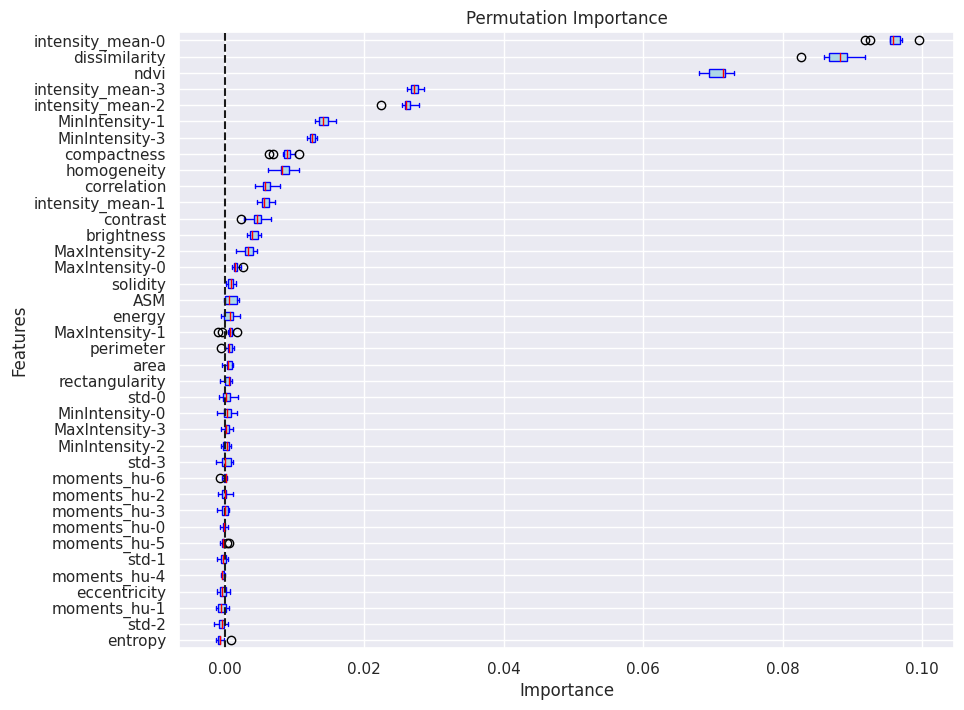
\includegraphics[width=1\linewidth]{images/permutation imp.png}
    \caption{How permuting different features will affect the accuracy score on the test data}
    \label{fig:permuatation importance}
\end{figure}
\section{CNN}
The classification report demonstrates that the simple CNN performs, on average, poorer than the Random Forest with an F1 score of 0.62. However, when examining its performance for each class, it performs relatively poorly compared to the Random Forest model. As observed with the Random Forest, spectral, textural, and geometric features all contributed to the model's predictive performance, albeit with varying degrees of importance. In contrast, CNNs predominantly rely on textural features for making predictions, which accounts for their comparatively lower performance in this context.

The model failed to identify any car classes, as indicated by the classification report, which shows 0 recall, 0 precision, and consequently, a 0 F1 score for the car class. This underscores the challenge of class imbalance that still persists. Despite the expectation that CNNs would perform better, the limited feature extraction capabilities of this CNN result in poorer performance. This limitation is illustrated in both the classification report and the confusion matrix.
\begin{figure}[h]
    \centering
    \begin{minipage}[b]{0.45\linewidth}
        \centering
        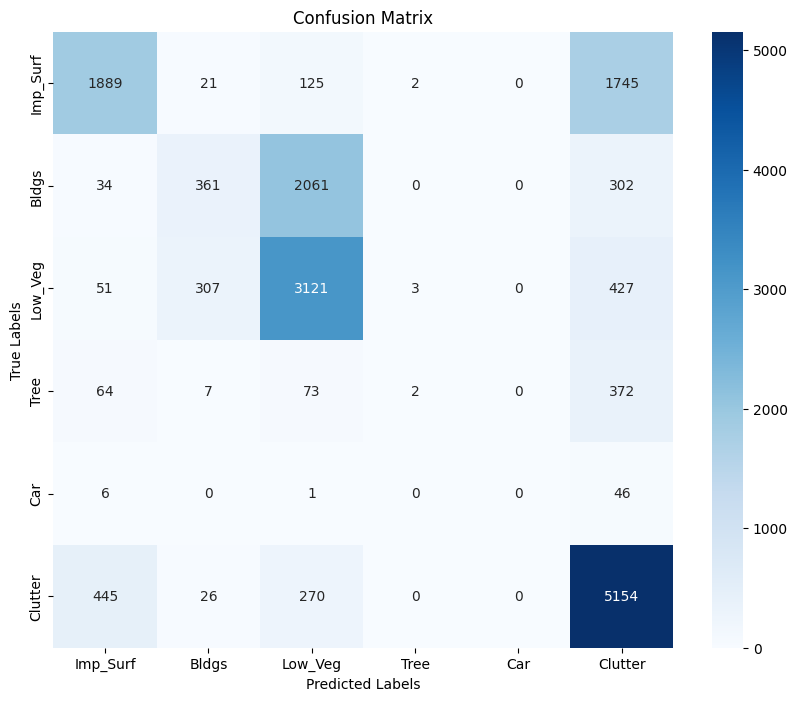
\includegraphics[height=5cm]{images/CNN CM.png} % Adjust the height as needed
        \caption{CNN Confusion matrix}
        \label{fig:CNN_CM}
    \end{minipage}
    \begin{minipage}[b]{0.45\linewidth}
        \centering
        \begin{tabular}{c|c|c|c|c}
        \hline
             Class & Precision & Recall & F1-Score & Support \\
             \hline
             Imp\_surf & 0.76 & 0.50 & 0.60 & 3782 \\
             Bldgs & 0.50 & 0.13 & 0.21 & 2758 \\
             Low\_Veg & 0.55 & 0.80 & 0.65 & 3909 \\
             Tree & 0.29 & 0.00 & 0.01 & 518 \\
             Car & 0.00 & 0.00 & 0.00 & 53 \\
             Clutter & 0.64 & 0.87 & 0.74 & 5895 \\
             \hline
             & & & & \\
             accuracy & & & 0.62 & 16915 \\
             macro avg & 0.46 & 0.38 & 0.37 & 16915 \\
             weighted avg & 0.61 & 0.62 & 0.58 & 16915 \\
        \end{tabular}
        \caption{CNN classification report}
        \label{tab:CNN_F1}
    \end{minipage}
\end{figure}


\section{GNN}
Still working on results that I can discuss for GNN